\section{From Measurements to a Migration Policy}
\label{sec:policy}

A scheduler deciding what to send needs three numbers per strategy: its bytes, whether those bytes drain in time, and
what the destination pays to recover. The first is exact for any architecture, since payload size depends only on
tensor shapes and codecs (Table~\ref{tab:bytes}). The second follows from the bandwidth. The third is what we
measured.

\textbf{Model.} Let a strategy $s$ have payload $B_s$ bytes and cost $\lambda_s$ steps of lost progress, and let the
job have bandwidth $w$, notice window $N$, step time $\tau$, $G$ accelerators at price $p$ per accelerator-hour, and
egress price $e$ per gigabyte. The drain takes $x_s = B_s / w$. If $x_s > N$ the payload does not leave in time; the
job restarts from its last periodic checkpoint and loses, in expectation, half a checkpoint interval. Otherwise the
migration costs
\begin{equation}
C_s = e\,B_s + G\,p\,(x_s + \lambda_s \tau),
\label{eq:cost}
\end{equation}
bytes on the wire plus accelerators idle during the drain and busy re-earning lost progress. The policy picks the
feasible strategy with the lowest $C_s$. A job that moves by choice, toward a cheaper region, moves only if the price
difference over its remaining steps exceeds $C_s$.

\textbf{An illustrative case.} Table~\ref{tab:policy} applies the model to the shapes of a \llamaParams{}-billion
parameter decoder~\cite{touvron2023llama2} with $G = 8$, $p = \$1.20$, $\tau = 6$\,s, $e = \$0.02$ per gigabyte and a
checkpoint every 1000 steps. \emph{These rows are extrapolations.} The byte counts are exact for those shapes. The
values of $\lambda_s$ are those measured at \paramsM{}M parameters for a migration at 60\% of the schedule, held
constant, and nothing here was trained at
that size. With that caveat the structure of the answer is robust to the exact $\lambda_s$, because it is driven by
feasibility. The full state, \llamaFullGB{}\,GB, needs \llamaFullDrain{}\,s at 10\,Gb/s. It fits a two-minute notice and
misses a thirty-second one, where a job that insists on it is thrown back to its last checkpoint. The quantised state
(\llamaQGB{}\,GB, \llamaQDrain{}\,s) still misses. The rank-one strategies (\llamaRankGB{}\,GB in \llamaRankDrain{}\,s,
or \llamaRankBfGB{}\,GB in \llamaRankBfDrain{}\,s with half-precision weights) fit with room to spare, and are the
ones Section~\ref{sec:main} found inside the noise floor. Fig.~\ref{fig:policy} shows the same boundary across
bandwidths.

\begin{table*}[t]
\caption{Policy output for a \llamaParams{}-billion-parameter model. \textbf{Extrapolated}: payload sizes are computed
from tensor shapes; recovery costs are those measured at \paramsM{}M parameters. Drain times are bytes over bandwidth
and exclude encoding.}
\label{tab:policy}
\centering
\footnotesize
\begin{tabular}{@{}lrrrcclrrr@{}}
\toprule
 & & & \multicolumn{2}{c}{\arm{full}} & & \multicolumn{4}{c}{Chosen strategy} \\
\cmidrule(lr){4-5}\cmidrule(l){7-10}
Scenario & Notice (s) & Gb/s & Drain (s) & Fits & Strategies that fit & Name & GB & Drain (s) & Cost (\$) \\
\midrule
\gen{tab_policy}
\bottomrule
\end{tabular}
\end{table*}

\begin{figure}[t]
\centering
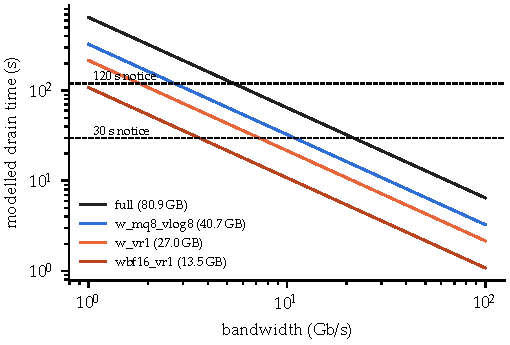
\includegraphics[width=\columnwidth]{policy}
\caption{Modelled drain time of four payloads for a \llamaParams{}-billion-parameter model against bandwidth
(extrapolated from tensor shapes; not measured). A payload above a dashed line does not leave within that notice.}
\label{fig:policy}
\end{figure}

\textbf{Reading the measurements as a rule.} Combined with Sections~\ref{sec:main}--\ref{sec:diag}, the policy reduces
to an order of preference. Send the quantised moments if they fit, since they cost nothing measurable. Otherwise drop
$m$ and send the rank-one sketch of $v$, with the weights in half precision if the window is still too short. If only
the weights can leave, the destination should re-estimate the second moment with a few frozen passes and leave the
first at zero, or, if it cannot spare the passes, build a new optimizer and ramp the learning rate again. It should not
keep the step counter over empty moments, and it should not re-estimate the first moment. Late in training the choice hardly matters and the smallest payload is the right
one; early in training it matters most (Section~\ref{sec:fork}).
